\documentclass[11pt,a4paper]{article}
\usepackage[margin=23mm]{geometry}
\usepackage{amsmath,booktabs,graphicx,xcolor}
\usepackage[colorlinks=true,linkcolor=teal,citecolor=teal,urlcolor=teal]{hyperref}
\title{A Small Experiment, Clearly Reported}
\author{Texite Demo Project}
\date{}
\begin{document}
\maketitle
\begin{abstract}
We compare three settings for a small prediction task. This note keeps the
question, metric, results, and limitations together. All values are synthetic
and illustrate a writing workflow, not a scientific finding.
\end{abstract}
\section{Question and method}
\label{sec:method}
Does using a larger training set improve prediction quality?
We compare the same model using 100, 300, and 500 training examples.
The evaluation metric is the mean absolute error:
\begin{equation}
  \operatorname{MAE}=\frac{1}{n}\sum_{i=1}^{n}|y_i-\hat{y}_i|.
  \label{eq:mae}
\end{equation}
A lower value is better. Table~\ref{tab:results} records the comparison.
\section{Results and limitations}
\label{sec:results}
The larger set has lower error in this synthetic comparison.
This does not establish a general result.

\begin{table}[htbp]
\centering
\caption{Illustrative results. All numbers are synthetic.}
\label{tab:results}
\begin{tabular}{lrr}
\toprule
Setting & Training examples & MAE \\
\midrule
Small & 100 & 0.42 \\
Medium & 300 & 0.31 \\
Large & 500 & 0.27 \\
\bottomrule
\end{tabular}
\end{table}

Before drawing a conclusion, repeat the experiment with several random
seeds and report the variation. The figure on the next page provides a
compact view of the same values.
\newpage
\section{A figure that stays connected}
\begin{figure}[htbp]
\centering
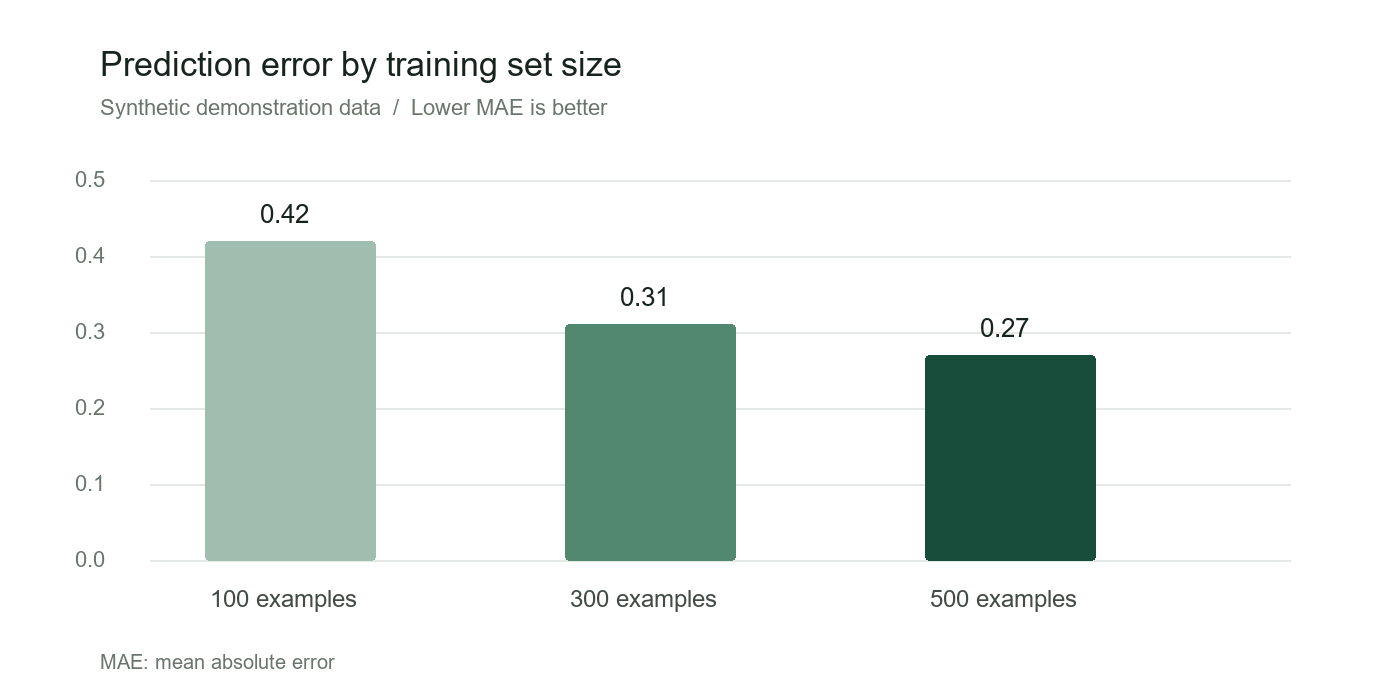
\includegraphics[width=.86\linewidth]{figures/comparison.png}
\caption{The same synthetic values as Table~\ref{tab:results}.}
\label{fig:comparison}
\end{figure}
Keep the data, figure, and text consistent when revising a result.
Equation~\ref{eq:mae} defines the metric; Section~\ref{sec:method} describes
the comparison. Cross-references update during compilation.
For background on document structure and references, see Lamport~\cite{latex1994}.
\subsection{Before sharing}
\begin{itemize}
\item Check that all citations and figure references resolve.
\item Describe limitations alongside the result.
\item Create a project backup before a substantial revision.
\end{itemize}
\bibliographystyle{plain}
\bibliography{references}
\end{document}
